
\documentclass[12pt,conference]{IEEEtran}

\usepackage{url}
\usepackage{graphicx}
\graphicspath{ {./images/} }
\usepackage{float}
\floatstyle{boxed} 
\restylefloat{figure}








\ifCLASSINFOpdf
  % \usepackage[pdftex]{graphicx}
  % declare the path(s) where your graphic files are
  % \graphicspath{{../pdf/}{../jpeg/}}
  % and their extensions so you won't have to specify these with
  % every instance of \includegraphics
  % \DeclareGraphicsExtensions{.pdf,.jpeg,.png}
\else
  % or other class option (dvipsone, dvipdf, if not using dvips). graphicx
  % will default to the driver specified in the system graphics.cfg if no
  % driver is specified.
  % \usepackage[dvips]{graphicx}
  % declare the path(s) where your graphic files are
  % \graphicspath{{../eps/}}
  % and their extensions so you won't have to specify these with
  % every instance of \includegraphics
  % \DeclareGraphicsExtensions{.eps}
\fi
% graphicx was written by David Carlisle and Sebastian Rahtz. It is
% required if you want graphics, photos, etc. graphicx.sty is already
% installed on most LaTeX systems. The latest version and documentation
% can be obtained at: 
% http://www.ctan.org/tex-archive/macros/latex/required/graphics/
% Another good source of documentation is "Using Imported Graphics in
% LaTeX2e" by Keith Reckdahl which can be found at:
% http://www.ctan.org/tex-archive/info/epslatex/
%
% latex, and pdflatex in dvi mode, support graphics in encapsulated
% postscript (.eps) format. pdflatex in pdf mode supports graphics
% in .pdf, .jpeg, .png and .mps (metapost) formats. Users should ensure
% that all non-photo figures use a vector format (.eps, .pdf, .mps) and
% not a bitmapped formats (.jpeg, .png). IEEE frowns on bitmapped formats
% which can result in "jaggedy"/blurry rendering of lines and letters as
% well as large increases in file sizes.
%
% You can find documentation about the pdfTeX application at:
% http://www.tug.org/applications/pdftex




\begin{document}

\title{SuRF: Implementation and RocksDB }

\author{\IEEEauthorblockN{Dhruvil Gandhi}
\IEEEauthorblockA{Seidenberg School of CSIS\\
Pace University\\
New York, NY\\
Email: dgandhi@pace.edu}
\and
\IEEEauthorblockN{Gunjan Asrani}
\IEEEauthorblockA{Seidenberg School of CSIS\\
Pace University\\
New York, NY\\
Email: gasrani@pace.edu}}

%special paper notices
\IEEEspecialpapernotice{This paper is a report of implementation of original paper: SuRF: Practical Range Query Filtering with Fast Succinct Tries}




% make the title area
\maketitle



\begin{abstract}
We present implementation of  Succinct Range Filter (SuRF), a fast and compact data
structure for approximate membership tests. It supports  single-key lookups and common
range queries: open-range queries, closed-range queries, and range
counts based on a new data structure called the Fast Succinct
Trie (FST) that matches the point and range query performance of
state-of-the-art order-preserving indexes, while consuming only
10 bits per trie node. The false positive rates in SuRF can be modified to satisfy different application needs.
We are evaluating SuRF in RocksDB as a replacement for its Bloom filters
to reduce I/O  by filtering requests before they access on-disk data
structures; the data is 100GB. The experiment uses YCSB data.
\end{abstract}

\begin{IEEEkeywords}
Filters, ARF, Bloom Filter, SuRF, rocksdb, FST
\end{IEEEkeywords}

\IEEEpeerreviewmaketitle



\section{Background}
% no \IEEEPARstart

There are different approximate query membership data structures designed and evaluated. Filters answers approximate membership of a query. Filters act as a guard when accessing data from devices which have high latency and limited bandwidth. Traditionally designed filters only support point queries, complete keys must be provided to the filter to test for membership. The paper \cite{1} proposes a new filter, SuRF or Succinct Range Filter which filters with both point queries (complete keys) and range queries(range of keys or partial keys). SuRF uses suffixed keys to improve false positive rate of the filter. The paper \cite{1} has experimentation implemented and evaluated for SuRF implemented in C++ \cite{3} and also tests performance \cite{4} of RocksDB \cite{2} by Facebook for point queries, range queries on single threaded and multi-threaded implementation. They evaluation states 1.5x to 5x improvement in RocksDB using SuRF over RocksDB with Bloom Filter. 

\section{Motivation}

SuRF is memory efficient \cite{1}, improves throughput and reduces I/O substantially. It seems promising technique to optimize database. To implement and re-evaluate the proposed solution, we tried to replicated and reproduce the results. RocksDB by facebook \cite{2} uses Bloom Filter, a point query filter. We try to replicate the experiment, replacing Bloom Filter with SuRF and compare them.


\section{Design}
The experiment code is available on github for SuRF \cite{3} and RocksDB \cite{2}. We first try to evaluate both.

The basic version of SuRF (SuRF-Base) stores the minimum length key prefixes such that it can uniquely identify each key. Specifically, SuRF-Base only stores an additional byte for each key
beyond the shared prefixes.

\begin{figure}[H]
\centering
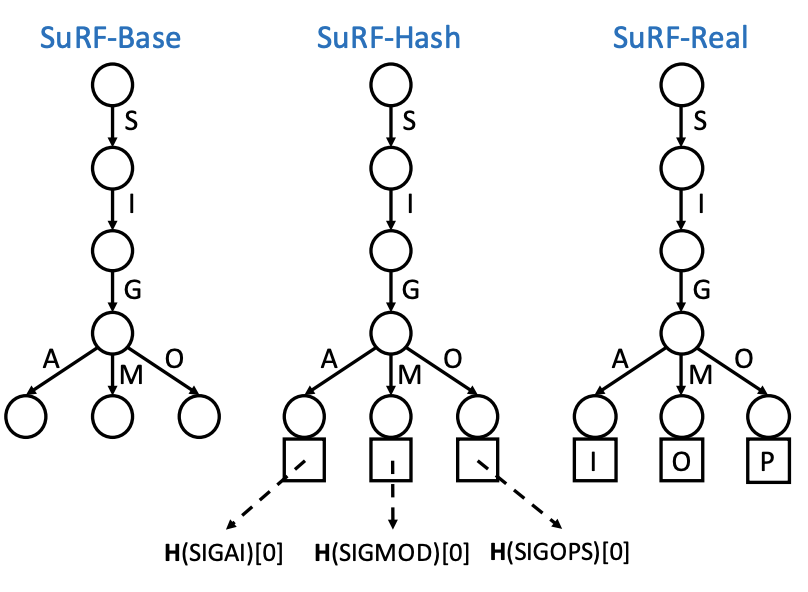
\includegraphics[width=2.5in]{surf}
\caption{Different SuRF versions}
\end{figure}

Different variations of SuRF are as
\begin{itemize}
	\item Basic SuRF
	\item SuRF with Hashed Key Suffixes
	\item SuRF with Real Key Suffixes
	\item SuRF with Mixed Key Suffixes
\end{itemize}

\section{Implementation}
We carried out a set of experimentation for both SuRF and the example application for RocksDB.
First we implemented SuRF basic code to compare Bloom Filter, No Filter and different variations of SuRF. Then we implemented different variants of SuRF with multi-threading support. Data from Yahoo's Cloud Serving Benchmark\cite{6} is used. The experiments is not implemented for email list. 

Our first run used the following configuration( t3.large on AWS \cite{5}):

\begin{itemize}
	\item2.5 GHz Intel Scalable Processor
	\item Intel AVX†, Intel AVX2†, Intel Turbo
	\item EBS Optimized(SSD for 300 I/Ops)
	\item Enhanced Networking†
	\item 2 vCPUs
	\item 8GB of memory
\end{itemize}
This configuration ran out of memory on first run. 

We switched to DigitalOcean with following configuration:
\begin{itemize}
	\item Intel(R) Xeon(R) CPU E5-2650L v3 1.80GHz
	\item 6vCPUs
	\item 16GB Multi-EEC 
	\item 160GB SSD
	\item 8GB of memory
\end{itemize}

\subsection{RocksDB Experiment}
After successful run of the SuRF code, we implemented the experiment carried out with RocksDB. The experiment implements SuRF in RocksDB and uses 100GB of data. Different queries are carried out  to test data with no-filter, bloom filter and SuRF. Throughput and seek timings in different scenarios recorded. The data is tested with 100\% positive and 50\% empty queries.

\section{Evaluation}

\subsection{SuRF Single Threaded}
When running single threaded operations,
the output was seen as:


\begin{table}[H]
\caption{Point Query Result}
\begin{tabular}{|c||c|c|}
\hline
Operation & Throughput & FPR\\
\hline  
Bloom Filter & 4.18142 & 0.00771089\\
\hline
SuRF & 2.25069 & 0.0414119\\
\hline
SuRFHash & 1.9057 & 0.00162597\\
\hline
SuRFReal & 1.95216 & 0.0054646\\
\hline
SuRFMixed & 1.61184 & 0.00951337\\
\hline
\end{tabular}
\end{table}




\subsection{SuRF Multi-Threaded}

When running different filters multi-threaded, we get the following throughput graph:

\begin{figure}[H]
\centering
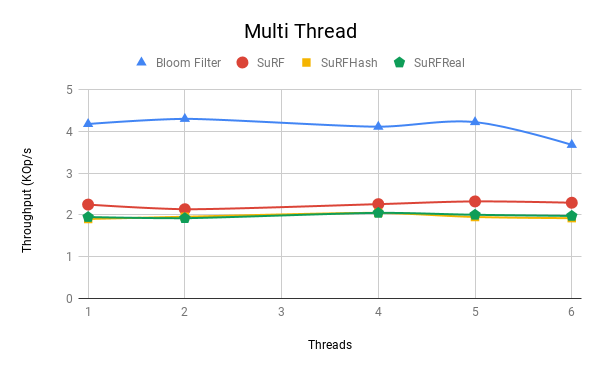
\includegraphics[width=3.5in]{thread}
\caption{Multi Threaded}
\end{figure}


\subsection {RocksDB}
When running with RocksDB, we first run it with point queries for No Filter, Bloom FIiter, and SuRF.
We observe that Bloom Filter has better throughput with Bloom Filter. This can be due to cached data. This needs to be examined again.

\begin{figure}[H]
	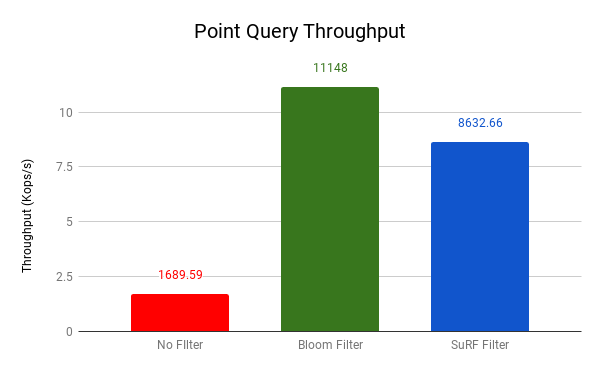
\includegraphics[width=3.5in]{point}
	\caption{Point Query RocksDB}
\end{figure}

We perform next set of evaluations with 50\% success range queries for No Filter, Bloom FIiter, and SuRF. We clear system cache before running each experiment.

\begin{figure}[H]
	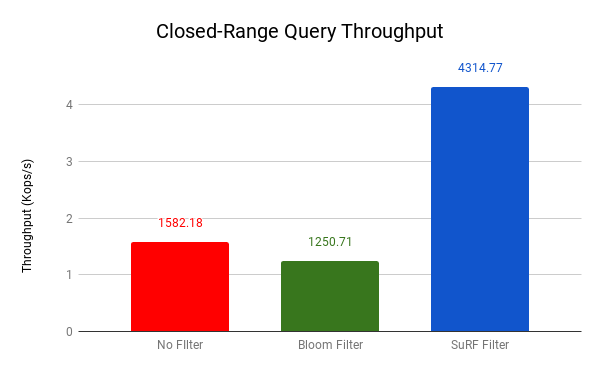
\includegraphics[width=3.5in]{cr}
	\caption{50\% empty results query RocksDB}
\end{figure}

We observe that SuRF significantly outperforms Bloom Filter and without filter operations. The I/O could not be obtained on the cloud due to logical disk structure naming. 


\subsection{Limitation}
The only limitation in implementation of this is there is lack of resources on the code developed.

\subsection {Comparision and Conclusion}
After implementing all the experiments, we conclude that SuRF is a promising filter for databases with improvements in throughput. In case of RocksDB, the I/O was monitored with monitoring metrics that DigitalOcean provides. The number of operations were reduced when using SuRF. We were unable to compare it to ARQ as the build step was not executed.

\section{Future Work}
We will like to implement more data-points and test for SuRF and compare it with ARF. We will like to run more tests with RocksDB. 

\section*{Acknowledgment}

We would like to thanks Dr. Juan Shan at Pace University. And DigitalOcean for final minutes changes in the billing plan to allow acclerated execution. The git repository for this work is available at \cite{7}

\begin{thebibliography}{r1}

\bibitem{1}
Huanchen Zhang, Hyeontaek Lim, Viktor Leis, David G. Andersen, Michael Kaminsky, Kimberly Keeton, and Andrew Pavlo. 2018.\emph{SuRF: Practical Range Query Filtering with Fast Succinct Tries}. In Proceedings of the 2018 International Conference on Management of Data (SIGMOD '18). ACM, New York, NY, USA, 323-336. DOI: \url{https://doi.org/10.1145/3183713.3196931}
%H.~Kopka and P.~W. Daly, \emph{A Guide to \LaTeX}, 3rd~ed.\hskip 1em plus
 % 0.5em minus 0.4em\relax Harlow, England: Addison-Wesley, 1999.  

\bibitem{2} 2018. RocksDB SuRF Implementation Github \url{https://github.com/efficient/rocksdb}  

\bibitem{3} 2018. SuRF Repository \url{https://github.com/efficient/SuRF}

\bibitem{4}2018.  RocksDB Repository by Facebook \url{https://github.com/facebook/rocksdb} 

\bibitem{5}2015. AWS EC2 intance \url{https://aws.amazon.com/ec2/instance-types/t3/} 

\bibitem{6}2018. Yahoo Cloud Serving Benchmark \url{https://research.yahoo.com/news/yahoo-cloud-serving-benchmark/?guccounter=1}

\bibitem{7}2018. SuRF-Report Github \url{https://github.com/dhruv857/rocksdb}

\bibitem{8}2018. Working rocksdb Repo \url{https://github.com/dhruv857/rocksdb}

\end{thebibliography}

\end{document}


